\section{Overview of the Universal Verification Methodology}\label{uvm}

The \emph{Universal Verification Methodology (UVM)} describes the Methodology to
verify \emph{integrated circuit (IC)} designs. It is standardized by Accellera \cite{uvm},
an independent standards organization. One of the key principles is to create
reusable verification environments and thereby enabling efficient development.
This is accomplished by using \emph{Universal Verification Components (UVCs)}.

\subsection{Universal Verification Components}\label{uvc}

A UVM testbench is composed of reusable and configurable UVCs, each
containing all functionalities to verify a single interface or module. The
structure of these components inside a UVM testbench is shown in figure
\ref{fig:UVM_testbench}.

\begin{figure}[htb]
 \centering
 %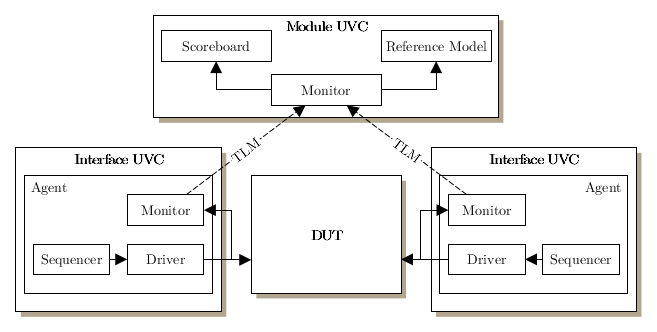
\includegraphics[width=1.0\textwidth,angle=0]{abb/UVM_testbench}
 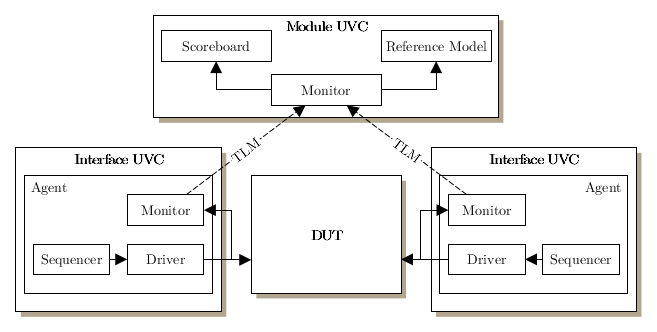
\includegraphics[scale=0.3]{abb/UVM_testbench}
 \caption{Structure of an UVM testbench}
\label{fig:UVM_testbench}
\end{figure}

\subsubsection{Interface UVC}\label{interface_uvc}

For each interface of an \emph{device under test (DUT)} an interface UVC has
to be created. Its purpose is to establish the communication between
the testbench and the signals of the DUT. More than one interface UVC can be
connected to the DUT. Its standard architecture contains the following elements \cite{uvm_sv}:

\begin{itemize}
  \item \textbf{Sequence item}\\
  Sequence items represent stimulus for an interface of the
  DUT or can be extracted from it for observation.
  The fields of a sequence item are derived from the attributes of the transaction.
  By this an object in a higher level of abstraction than the signals of the
  DUT themselves is created.
  \item \textbf{Sequencer/Sequence Driver}\\
  The sequencer in \emph{UVM-SystemVerilog} (UVM-SV) respectively the sequence
  driver in UVM-\textit{e} \cite{uvm_e} is a stimulus generator. It creates random
  stimulus by executing sequences. These sequences either generate one or more
  sequence items or other sequences.
  \item \textbf{Driver/Bus Functional Model (BFM)}\\
  The driver in UVM-SV respectively BFM in UVM-\textit{e} \cite{uvm_e} receives a sequence
  item from a sequencer or sequence driver. Then the extracted attributes are
  used to drive the signals of the DUT. So the active functionalities of an
  interface UVC are split between the transaction-level sequencer or sequence
  driver and the signal-level driver or BFM.
  \item \textbf{Monitor}\\
  The monitor basically inverts the functionality of a driver or BFM. It samples
  the signal of the DUT and generates sequence items. Additionally it collects coverage
  and performs checking. The monitor is a passive entity and does not drive any
  signals of the DUT.
  \item \textbf{Collector} (optional)\\
  Just like dividing stimuli generation into transaction-level and signal-level
  the same can be done for sampling. Thereby the monitor furthermore collects
  coverage and performs checking, but the signal-level functionality is
  transferred into another unit called collector. This partitioning is optional
  and not mandatory for UVM.
  \item \textbf{Agent}\\
  Agents encapsulate sequencers/sequence drivers, drivers/BFMs and monitors to
  ensure reusability. They can either be active and drive the signals of the DUT
  or passive and monitor the DUT's interface while other DUTs drive the
  signals. The active elements of an agent are the sequencer/sequence driver as
  well as the driver/BFM and passive ones are the collector and the monitor. The
  passive elements of an UVC are also used when the agent is configured as
  active. UVCs can contain more than one agent, for example master or slave
  agents.
  \item \textbf{Environment}\\
  The environment is the top-level entity of the UVC. It contains all agents as
  well as configuration properties, which are used to customize the UVC and
  therefore make it reusable.
\end{itemize}

\subsubsection{Module UVC}\label{module_uvc}

Because an interface UVC can only capture information of a single interface,
module UVCs are necessary to verify data across multiple interfaces. They are
connected to interface UVCs via \emph{Transaction-Level Modeling (TLM)
ports} (see section \ref{tlm}). The received data are then processed in a
scoreboard or reference model to check the behavior over multiple interfaces.
Thereby the DUT is seen as a black box. Meaning its internal structure is not
visible to the testbench. So the module UVC describes this internal structure
and uses this information to verify the interaction of multiple interfaces of
the DUT. Since it is a passive element, it can be reused in system-level
verification \cite{uvm}.

\subsection{Data Communication between Components}\label{tlm}

To communicate between UVCs TLM ports are used, which improve reusability \cite{uvm_sv}. With
them transactions are exchanged without explicit type conventions via a
method call, that is bind to the TLM port. It is even possible to communicate
between different verification languages, if they include TLM ports for
compatible transactions. Examples for verification languages supporting TLM ports are UVM-SystemVerilog, UVM-SystemC and
UVM-\textit{e}. Communication between verification languages is discussed in more
detail in section \ref{ml_tlm}.
